\documentclass{article} % For LaTeX2e


%%%
% STANDARD PREAMBLE
%%%
%https://tex.stackexchange.com/questions/68821/is-it-possible-to-create-a-latex-preamble-header
\usepackage{/Users/miw267/Repos/latex_preamble/preamble}


%%%
% SPECIAL TO THIS DOC
%%%

\usepackage{amsthm}
\usepackage{tcolorbox}
\tcbuselibrary{theorems}

% Colored theorems
\let\theorem\relax
\let\endtheorem\relax
\newtcbtheorem[number within=section]{theorem}{Theorem}
{colback=blue!5,
 colframe=blue!70!black,
 fonttitle=\bfseries}{thm}
 
 %%%
 % START DOC
 %%%
 
\title{CSCI 546 (Spring 2026): Midterm Study Guide}
%\author{Mike Wojnowicz}


\begin{document}

\maketitle

\begin{abstract}
Note: the reference material is a work in progress.
\end{abstract}


\section{Midterm Overview}

The midterm will present 8 questions, of which you will need to answer 5.  In particular, the midterm will present 3 questions on probability fundamentals (of which you should answer 2), 3 questions on Markov Chains (of which you should answer 2), and 2 questions from diffusion processes (of which you should answer 1).  The questions presented will be a subset of the bank below.


\subsection{Scaffolding: Example Question}

On the exam, I'll provide hints about how to solve each question.   For example, a sample exam question might look like this:

\begin{enumerate}
	\item (Chang Sec 5.1) \textbf{Covariance of Brownian Motion.}  Prove that for standard Brownian motion, $\Cov(W_s, W_t) = s \wedge t.$ (Recall the notation that $s \wedge t := \min(s,t)$).
	\begin{itemize}
	\item  Hint: Assuming $s<t$, you can write $W_t = (W_s-W_0) + (W_t-W_s)$ and then apply the independent increments property. (See the definition for standard Brownian motion in the reference section.) %so consider writing $W_t = W_s + (W_t-W_s)$ if $s<t$.
	\item Hint: Use the additivity of covariance: $\Cov(X+Y,Z) = \Cov(X,Z)+\Cov(Y,Z)$.
	\item Hint: Use that $\Cov(X,X)=\Var(X)$.
	\end{itemize}
\end{enumerate}

\section{Probability Fundamentals}



\begin{enumerate}
\item (1.3.2) A fair coin is tossed repeatedly. Show that, with probability one, a head turns up sooner or later.  (Similarly, any finite sequence of heads or tails occurs eventually with probability one. However, you do not need to show this.) 
\item (1.4.5i) \textbf{The Monty Hall Problem: goats and cars.} In a game show, you have to choose one of three doors. One conceals a new car, two conceal old goats. You choose, but your chosen door is not opened immediately. Instead, the presenter opens another door, which reveals a goat.  He offers you the opportunity to change your choice to a third door (unopened and so far unchosen).  Let $p$ be the (conditional) probability that the third door conceals the car.  Show that $p=2/3$, assuming that the presenter is determined to show you a goat (show with a choice of two, he picks one at random).
\item (1.5.9) Two fair dice are rolled. Show that the event that their sum is 7 is independent of the score shown by the first die.
\item (1.7.2) A hand of 13 cards is dealt from a normally shuffled pack of 52 cards. What is the probability that the hand contains exactly one ace given that it contains exactly two kings? 
\item  (2.1.6) \textbf{Uniform Distribution.}  A random variable that is equally likely to take any value in a finite set $S$ is said to to have the \textit{uniform distribution} on $S$.  If $U$ is such a random variable and $\emptyset \neq R \subseteq S$, show that the distribution of $U$ conditional on $\set{U \in R}$ is uniform in $R$.
\item  (CH 2) \textbf{The Dice DJ.}  A DJ has a strange music mixer with three independent fair six-sided dice:
	\noindent
	\begin{itemize} 
	\item Die A controls bass,
	\item Die B controls treble,
	\item Die C controls tempo.
	\end{itemize}
Let $X = \text{max}(A,B,C)$ be the loudest setting reached by any dial. (a) What is the distribution of $X$? (b) What is the probability that the system hits level 5 or higher?
\item (3.2.1) Let $X$ and $Y$ be independent random variables, each taking the values -1 and 1 with probability $\frac{1}{2}$, and let $Z=XY$. Show that $X,Y$ and $Z$ are pairwise independent. Are they independent?
\item (3.5.2) In your pocket is a random number $N$ of coins, where $N$ has the Poisson distribution with parameter $\lambda$.  You toss each coin once, with heads showing with probability $p$ each time.  Show that the total number of heads has the Poisson distribution with parameter $\lambda p$.
\item (3.11.16) Let $X$ and $Y$ be independent Bernoulli random variables with parameter $\frac{1}{2}$.  Show that $X+Y$ and $|X-Y|$ are dependent though uncorrelated.
\item (3.7.6a) Let $X_1, X_2, \hdots$ be identically distributed random variables with mean $\mu$ and variance $\sigma^2$, and let $N$ be a random variable taking values in the non-negative integers and independent of the $X_i$.  Let $S=X_1+X_2+\cdots+X_N$.    Show that $\E[S \mid N] = \mu N$, and deduce that $\E[S]=\mu \E[N]$. 
\item (4.14.5b) Prove that the exponential distribution is memoryless.  (Note: the exponential distribution is the \textit{only} continuous distribution with this property!)
\item (4.5.5a) Let $X$ and $Y$ be independent continuous random variables.  Show that
\[ \E[g(X)h(Y)]= \E[g(X)] \E[h(Y)] \]
whenever these expectations exist.  %If $X$ and $Y$ have the exponential distribution with parameter 1, find $\E[e^{\half (X+Y)}]$.
\item (4.5.4) Let $X$ and $Y$ be independent random variables each having the uniform distribution on $[0,1]$.  Let $U=\text{min}\set{X,Y}$ and  $V=\text{max}\set{X,Y}$.  Find $\E[U]$ and $\E[V]$, and then calculate $\Cov[U,V]$.   Are $U$ and $V$ independent? 
\item (Sec 4.6) \textbf{Conditional distributions.} Suppose $X,Y$ has the joint density

\[ f_{X,Y}(x,y) =
\begin{cases}
2, & 0 < x < y < 1, \\
0, & \text{otherwise}.
\end{cases}
\]
(a) Find the \textit{marginal density} $f_Y(y)$. (b) Compute the \textit{conditional density} $f_{X\mid Y}(x \mid y)$. 
\end{enumerate}

%\appendix
\section{Markov Chains}

\begin{enumerate}
\item (6.1.2) \textbf{Identifying Markov Chains.} A die is rolled repeatedly.  Which of the following are Markov chains? For those that are, supply the transition matrix
	\begin{itemize}
	\item[(a)] The largest number $X_n$ shown up to the $n$-th roll.
	\item[(b)] The number $N_n$ of sixes in $n$ rolls.
	\item[(c)] At time $r$, the time $C_r$ since the most recent six.
	\item[(d)] At time $r$, the time $B_r$ until the next six.
	\end{itemize}
\item (Sec 6.2) \textbf{Random walk: recurrence and transience.} Show that a simple random walk is periodic with period 2.  Then show that a simple random walk is recurrent if $p=\half$ but transient if $p \neq \half$.  
	\begin{itemize}
	\item Hint: Use Stirling's formula: $n! \sim \sqrt{2 \pi n} \, \big(\frac{n}{e}\big)^n$. 
	\item For additional help, see slide 22 \href{https://www.stat.uchicago.edu/~yibi/teaching/stat317/2021/Lectures/Lecture3.pdf}{\blue{\underline{here.}}} 
	\end{itemize}
\item (6.4.6) \textbf{Random walk on a graph.} A particle performs a random walk on a vertex set of a connected graph $G$, which for simplicity we assume to have neither loops nor multiple edges.  At each stage it moves to a neighbor of its current position, each such neighbor being chosen with equal probability.  If $G$ has $\eta (< \infty)$ edges, show that the stationary distribution is given by $\pi_v = d_v/(2\eta)$, where $d$ is the degree of vertex $v$.
\item (6.4.11a) \textbf{Bow tie.} A particle performs a random walk on a bow tie ABCDE drawn beneath, where $C$ is the knot.  From any vertex its next step is equally likely to be any neighboring vertex.  Initially it is at A.  Find the expected value of the time of first return to A.
\begin{center}
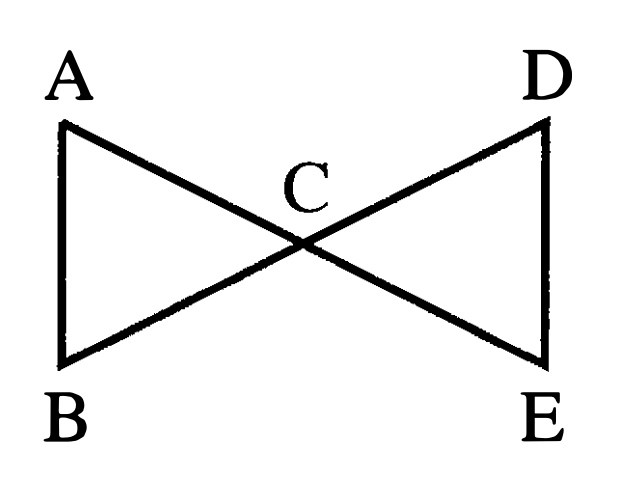
\includegraphics[width=.25\textwidth]{images/bow_tie.png}	
\end{center}
\item (6.5) \textbf{The Ehrenfest model.} Find the stationary distribution for the Ehrenfest model of diffusion.   (Hint: Rather than solve the equation $\+\pi = \+\pi \+P$, consider that the diffusion model might be reversible in equilibrium.   That is, look for solutions to the detailed balance equation $\pi_i p_{ij} = \pi_j p_{ji}$.)
\item (6.9) \textbf{Holding times.} Let $X$ be a continuous time Markov chain.  Let $X(0)=i$, and $U_0=\inf\set{t: X(t)\neq i}$ be the time of the first change in value.  Show that $U_0$ has the exponential distribution. %(Hint: Use this result from 4.14.5a:  Let $g: [0,\infty) \to [0,\infty)$ be such that $g(s+t)=g(s)g(t)$ for $s,t \geq 0$. If $g$ is monotone, then $g(s)=e^{\mu s}$ for some $\mu$.)
\end{enumerate}


\section{Diffusion Processes}

\begin{enumerate}
	\item (Chang Sec 5.1) \textbf{Covariance of Brownian Motion.}  Prove that for standard Brownian motion, $\Cov(W_s, W_t) = s \wedge t.$ (Recall the notation that $s \wedge t := \min(s,t)$).
\item (Chang Sec 5.6) \textbf{Brownian Bridge.}  Verify that the below is an easy way to manufacture a Brownian bridge from standard Brownian motion:
	\[ X(t) = W(t)-t W(1), \qquad \text{for } 0 \leq t \leq 1.\]
\item (Chang Sec 6.1) \textbf{Discretized Diffusion.} Let $\Delta X = X_{t + \Delta t} - X_t$ be a small change in the diffusion process. Then per Chang pp.180, we have
	\begin{align*}
	 \Delta X = \mu(X_t) \Delta t + \sigma(X_t) \, \sqrt{\Delta t} \, Z  \qquad Z, \sim N(0,1)
	\end{align*}
	%
	Show that as $\Delta t \downarrow 0$.
	\begin{align*}
	\E[\Delta X \mid X(t)=x] = \mu(x) \Delta t + o(\Delta t)\\	
	\E[(\Delta X)^2 \mid X(t)=x] = \sigma^2(x) \Delta t + o(\Delta t)
	\end{align*}
\item (Gautam Iyer, \textit{\href{https://www.math.cmu.edu/~gautam/sj/teaching/2021-22/944-scalc-finance1/pdfs/ch3-int.pdf}{\underline{\blue{Stochastic Integration. (Lecture notes.)}}}}) \textbf{Total Variation of Brownian Motion.} Let $W$ be Brownian motion, and let $\Delta W_{k,n}$ denote the increment 
	\[ \Delta W_{k,n} = W \bigg( \frac{kt}{n} \bigg) -  W \bigg( \frac{(k-1)t}{n} \bigg)\] 
	over the $k$-th bin $(k=1, \hdots, n)$ of the uniform partition of $[0,t]$ with mesh size $\Delta t=\frac{t}{n}$.    Let $T_n = \sum_{k=1}^{n} |\Delta W_{k,n}|$.  Compute $\lim_{n \to \infty} \E[T_n]$.  
	\item (Chang Sec 6.7) \textbf{Quadratic variation of Brownian motion.} Let $W$ be Brownian motion, and let $\Delta W_{k,n}$ denote the increment 
	\[ \Delta W_{k,n} = W \bigg( \frac{kt}{n} \bigg) -  W \bigg( \frac{(k-1)t}{n} \bigg)\] 
	over the $k$-th bin $(k=1, \hdots, n)$ of the uniform partition of $[0,t]$ with mesh size $\Delta t=\frac{t}{n}$.  Let $Q_n = \sum_{k=1}^{n} (\Delta W_{k,n})^2$.  Compute $\lim_{n \to \infty} \E[Q_n]$.
\item (Chang Sec 6.9) \textbf{Geometric Brownian motion.} Let $X_t$ be a stochastic process governed by the It\^{o} SDE 
	\[dX_t = \mu dt + \sigma dW_t.\]  
	Define a new stochastic process by $Y_t = e^{X_t}.$ Use It\^{o} chain rule (also called It\^{o}'s Lemma) to show that $Y_t$ is a geometric Brownian motion, and find the infinitesimal parameters of $Y_t$ with respect to the infinitesimal parameters of $X_t$. Provide an interpretation of the infinitesimal parameters.
\item (Gautam Iyer, \textit{\href{https://www.math.cmu.edu/~gautam/sj/teaching/2021-22/944-scalc-finance1/pdfs/ch3-int.pdf}{\underline{\blue{Stochastic Integration. (Lecture notes.)}}}}, Exercise 6.1.) \textbf{Integrating Brownian motion against Brownian motion.} Use It\^{o} chain rule (also called It\^{o}'s Lemma) to verify the identity
	\[ \int_0^T W \, dW = \half \bigg( W^2(T) - T \bigg). \]
\end{enumerate}

\appendix

\section{Reference Material}

Note: this is a work in progress.

%\subsection{Markov Chains}
%
%\begin{enumerate}
%	\item 
%\end{enumerate}

\subsection{Diffusion Processes}

\begin{enumerate}
\item A \textbf{stochastic process} $\set{X(t): t \in \mathcal{T}}$ is a collection of random variables over some index set $\mathcal{T} \subset \R$.
\item A \textbf{Gaussian process} $\set{X(t): t \geq 0}$ is a stochastic process such that for all numbers $n=1,2,\hdots$ and all times $t_1, t_2, \hdots t_n$, the random vector $\big( X(t_1), X(t_2), \hdots, X(t_n) \big)$ has a joint normal distribution.
\item A \textbf{standard Brownian motion} $\set{W(t): t \geq 0}$ is a stochastic process having
\begin{itemize}
\item[(i)] continuous paths,
\item[(ii)] stationary, independent increments, and
\item[(iii)] $W(t) \sim N(0,t)$ for all $t \geq 0$.
\end{itemize} 
\item A \textbf{standard Brownian Bridge} is a Gaussian process $X$ with continuous paths, mean 0, and covariance function $\Cov(X_s, X_t)=s(1-t)$ for $0 \leq s \leq t \leq 1$.

\item \textbf{Little-o notation.} Let $f(x)$ and $g(x)$ be functions defined on some neighborhood of $x_0$. We write
	$f(x) = o(g(x))$ as $x \to x_0$ if 
	\[
	\lim_{x \to x_0} \frac{f(x)}{g(x)} = 0.
	\]
Equivalently, $f(x)$ becomes negligible relative to $g(x)$ as $x$ approaches $x_0$.
\item \textbf{Infinitesimal parameters.} Consider a stochastic differential equation (SDE) of the form  
%
\begin{align*}
dX = \mu(X) \, dt + \sigma(X) dW.
\end{align*}
Then we have
%
\begin{align*}
\E[X(t+h)-X(t) \mid X(t)=x] &= \mu(x)h + o(h), \\
\intertext{and}
\Var[X(t+h)-X(t) \mid X(t)=x] &= \sigma^2(x)h + o(h). \\	
\end{align*}
%
Terms like \enquote{infinitesimal mean function} or \enquote{infinitesimal drift}  are used for $\mu(\cdot)$, and  $\sigma^2(\cdot)$ has names like \enquote{infinitesimal variance function} or \enquote{diffusion function}.
\item \textbf{It\^{o}'s Lemma (heuristic statement, special case.)} 
Let  $X(\cdot)$ be a 1-dimensional real-valued stochastic process which solves the following SDE  
%
\begin{align*}
dX = b \, dt + dW,
\end{align*}
where $W$ is 1-dimensional Brownian motion. Let $u: \R \to \R$ be a given smooth function, $u=u(x)$.  Consider the SDE 
\[ Y(t) \defeq u(X(t)), \qquad (t \geq 0). \]
Then 
\[ dY = \bigg(u'b + \red{\half u''} \bigg) dt + u' dW,  \]
where here we use the notation ${}^\prime = \frac{d}{dx}$.
%TODO (Diffusion): Def of stationary increments, independent increments.
%TODO (Markov Chain): Ehrenfest model. Recurrent, transient.
\end{enumerate}


\end{document}


